%%%%%%%%%%%%%%%%%%%%%%%%%%%%%%%%%%%%%%%%%%%%%%%%
\input{./format/preamble.ltx} 

%%%%%%%%%%%%%%%%%%%%%%%%%%%%%%%%%%%%%%%%%%%%%%%%
% as needed, comment the following lines by prefixing the percent sign at the start of the line

\PutLineNumberstrue % comment only if line numbers will not be put at the left side margin; this also will turn off certain  preparation guides 

\Figurestrue % comment only if figures will not be rendered 

\GroupIDtrue % comment if no group ID

\ResultDiscusstrue % comment to disable results and discussions

\Conctrue % comment to disable conclusions

\Finishedtrue % comment only if you will not be printing your manuscript prior to final hard binding, i.e. you are not told by your thesis adviser that you have passed, and you have no submitted the requirements

%\Gradtrue % comment to disable graduate school format

\PhDtrue % comment to disable PhD dissertation format

\PubListtrue % comment to disable publication list

\Vitatrue % comment to disable author(s) vita

\Indextrue % comment to disable index 

%%%%%%%%%%%%%%%%%%%%%%%%%%%%%%%%%%%%%%%%%%%%%%%%
% document IDs

\newcommand{\documentType}{Thesis Proposal} % specify if dissertation, thesis, project, dissertation proposal, thesis proposal, project proposal 
\newcommand{\college}{Gokongwei College of Engineering}
\newcommand{\department}{Department of Electronics and Communications Engineering} 
\newcommand{\degreeType}{Bachelor of Science} 
\newcommand{\degree}{Computer Engineering}
\newcommand{\degreeAbbrv}{BS-CPE}

\newcommand{\documentAdviserTitle}{Engr.} 
\newcommand{\documentAdviser}{Melvin K. Cabatuan}

\newcommand{\examinerChairTitle}{Dr.} 
\newcommand{\examinerChair}{Donabel D. Abuan}

% Sort in alphabetically ascending manner the surnames of the examiners
\newcommand{\examinerATitle}{Engr.} 
\newcommand{\examinerA}{Argel A. Bandala}

\newcommand{\examinerBTitle}{Engr.} 
\newcommand{\examinerB}{Mark Lorenze D. Torregoza}


\newcommand{\deanTitle}{Dr.} 
\newcommand{\deanName}{Jonathan R. Dungca}

\newcommand{\groupID}{ESG-04} % group ID number is for undergraduates as of this formatting

\newcommand{\numberOfAuthors}{4} % adapt the number of names below accordingly and sort the sunames in alphabetically ascending manner, like the given example

\defineAuthor{surname1}{Castillo}
\defineAuthor{firstname1}{Karlos Leo F.}

\defineAuthor{surname2}{Del Rosario}
\defineAuthor{firstname2}{Aldwin Jocep C.}

\defineAuthor{surname3}{Jarabelo}
\defineAuthor{firstname3}{Adrian Benjamin S.}

\defineAuthor{surname4}{Uy}
\defineAuthor{firstname4}{Charleston Franklin C.}

\newcommand{\documentTitle}{Student Tracking System Using Radio~Frequency~Identification} % put tilde (~) between words to indicate non-breaking adjacent words

\newcommand{\keywords}{alloy system, characterization, InP, InGaAs}

\newcommand{\approvalDate}{April~27,~\the\year} % put here the date when all examiners and/or their approved representative have given their approval; do not remove the tildes in order to not break the date; the submission deadline can also be placed as the date

\hyphenation{op-tical net-works semi-conduc-tor evi-dent re-la-tive re-si-den-tial po-la-ri-za-tion so-lu-tion/s} % for correcting bad hyphenation

%%%%%%%%%%%%%%%%%%%%%%%%%%%%%%%%%%%%%%%%%%%%%%%%
\input{./format/postamble.ltx} 

%%%%%%%%%%%%%%%%%%%%%%%%%%%%%%%%%%%%%%%%%%%%%%%%
% for placing user-defined-ambles

\DeclareMathAlphabet{\mathitbf}{OML}{cmm}{b}{it} %for math italic bold 

%%%%%%%%%%%%%%%%%%%%%%%%%%%%%%%%%%%%%%%%%%%%%%%%
% \includeonly{} is for specifying which files to include; if you only want to work on one or few chapters, you can only include those chapters, which will speed up the document build; advantage: fast if you have a large number of images in your results chapter, which you do not need when you are working on other chapters; you can still reference all the figures in the omitted chapter, as long as you have previously LaTeX-built the entire document

% Note that the file names below must correspond to those names inside \include{} in the \begin{document} ... \end{doument} enviroment, otherwise the chapter will not be included

%  the excludeonly package provides the logically opposite command: \excludeonly{<file list>}

\includeonly{
introduction,
literature_review,
%theoretical_considerations,
%design_considerations,
%methodology,
%results_and_discussion,
%conclusions,
answers_to_questions,
usage_examples,
publication,
vita,
}

%%%%%%%%%%%%%%%%%%%%%%%%%%%%%%%%%%%%%%%%%%%%%%%%
\begin{document}
\pagenumbering{roman} % roman page numbering starts here

%%%%%%%%%%%%%%%%%%%%%%%%%%%%%%%%%%%%%%%%%%%%%%%%
\input{./format/pre_toc.ltx}
\cleardoublepage

%%%%%%%%%%%%%%%%%%%%%%%%%%%%%%%%%%%%%%%%%%%%%%%%
\begin{SingleSpace}
\tableofcontents
\cleardoublepage

%%%%%%%%%%%%%%%%%%%%%%%%%%%%%%%%%%%%%%%%%%%%%%%%
\listoffigures
\cleardoublepage

%%%%%%%%%%%%%%%%%%%%%%%%%%%%%%%%%%%%%%%%%%%%%%%%
\listoftables
\cleardoublepage

%%%%%%%%%%%%%%%%%%%%%%%%%%%%%%%%%%%%%%%%%%%%%%%
\phantomsection
\addcontentsline{toc}{chapter}{Abbreviations}
{
	\printterms[database=abbreviation, style=indexalign, prelocation=dotfill, location=first, columns=1, postname=\hspace{3em}]
	\thispagestyle{plain}
}	
\cleardoublepage

%%%%%%%%%%%%%%%%%%%%%%%%%%%%%%%%%%%%%%%%%%%%%%%
\phantomsection
\addcontentsline{toc}{chapter}{Notation}
{
	\printterms[database=notation, style=indexalign, prelocation=dotfill, location=first, columns=1, postname=\hspace{3em}]
	{
	\vspace{3ex}
	\noindent Throughout this \MakeTextLowercase{\documentType}, mathematical notations conform to ISO~80000-2 standard, e.g. variable names are printed in italics, the only exception being acronyms like e.g. $\mathrm{SNR}$, which are printed in regular font.  Constants are also set in regular font like $\mathrm{j}$.  Functions are also set in regular font, e.g. in $\sin \left( \cdot \right)$.  Commonly used notations are $t$, $f$, $\mathrm{j} = \sqrt{-1}$, $n$ and $\exp \left( \cdot \right)$, which refer to the time variable, frequency variable, imaginary unit, $n$th variable, and exponential function, respectively.
	}
	\thispagestyle{plain}
}
\cleardoublepage

%%%%%%%%%%%%%%%%%%%%%%%%%%%%%%%%%%%%%%%%%%%%%%%%
\phantomsection
\addcontentsline{toc}{chapter}{Glossary}
{
	\printterms[database=glossary, style=gloss, prelocation=dotfill, location=first, columns=1, postname=\hspace{1em}]
	\thispagestyle{plain}
}
\cleardoublepage

%%%%%%%%%%%%%%%%%%%%%%%%%%%%%%%%%%%%%%%%%%%%%%%%
\lstlistoflistings
\cleardoublepage
\end{SingleSpace}

%%%%%%%%%%%%%%%%%%%%%%%%%%%%%%%%%%%%%%%%%%%%%%%%
\pagenumbering{arabic} % arabic page numbering starts here
\chapter{Introduction}
\label{ch:intro}
\startcontents[chapters]
\begin{SingleSpace}	
	\Mprintcontents  % for creating an actual mini TOC for this chapter
\end{SingleSpace}
\include{introduction}
\stopcontents[chapters]
\cleardoublepage

%%%%%%%%%%%%%%%%%%%%%%%%%%%%%%%%%%%%%%%%%%%%%%%%
\chapter{Literature Review} 
\label{ch:litrev} 
\startcontents[chapters]
\begin{SingleSpace}	
	\Mprintcontents 
\end{SingleSpace}
\include{literature_review}
\stopcontents[chapters]
\cleardoublepage


%%%%%%%%%%%%%%%%%%%%%%%%%%%%%%%%%%%%%%%%%%%%%%%%

%\chapter{Theoretical Considerations}
%\chaptermark{Theoretical Considerations} % uncomment this and put a shorter version of the chapter title for the TOC and chapter markings (i.e., header or footer)
%\label{ch:theorycon}
%\startcontents[chapters]
%\begin{SingleSpace}	
%	\Mprintcontents 
%\end{SingleSpace}
%\include{theoretical_considerations}
%\stopcontents[chapters]
%\cleardoublepage

%%%%%%%%%%%%%%%%%%%%%%%%%%%%%%%%%%%%%%%%%%%%%%%%
%\chapter{Design Considerations} 
%\label{ch:designcon} 
%\startcontents[chapters]
%\begin{SingleSpace}	
%	\Mprintcontents 
%\end{SingleSpace}
%\include{design_considerations}
%\stopcontents[chapters]
%\cleardoublepage

%%%%%%%%%%%%%%%%%%%%%%%%%%%%%%%%%%%%%%%%%%%%%%%%
%\chapter{Methodology} 
%\label{ch:method} 
%\startcontents[chapters]
%\begin{SingleSpace}	
%	\Mprintcontents 
%\end{SingleSpace}
%\include{methodology}
%\stopcontents[chapters]
%\cleardoublepage

%%%%%%%%%%%%%%%%%%%%%%%%%%%%%%%%%%%%%%%%%%%%%%%%
%\ifResultDiscuss 
%	\chapter{Results and Discussion} 
%	\label{ch:result_discuss} 
%	\startcontents[chapters]
%	\begin{SingleSpace}	
%		\Mprintcontents 
%	\end{SingleSpace}
%	\include{results_and_discussion}
%	\stopcontents[chapters]
%	\cleardoublepage
%\fi

%%%%%%%%%%%%%%%%%%%%%%%%%%%%%%%%%%%%%%%%%%%%%%%%
%\ifConc
%	\chapter{Conclusions, Recommendations, and Future Directives} 
%	\label{ch:conc} 
%	\startcontents[chapters]
%	\begin{SingleSpace}	
%		\Mprintcontents 
%	\end{SingleSpace}
%	\include{conclusions}
%	\stopcontents[chapters]
%	\cleardoublepage
%\fi

%%%%%%%%%%%%%%%%%%%%%%%%%%%%%%%%%%%%%%%%%%%%%%%
\renewcommand{\UrlFont}{\normalfont}
%\bibliographystyle{IEEEtr} % for IEEE referencing format
\bibliographystyle{apalike} % for APA referencing format
\begin{SingleSpace}
	{\small \bibliography{references}}
\end{SingleSpace}
\vfill
\begin{flushright}
Produced: \usdate\today, \currenttime \\
\end{flushright}
\cleardoublepage 

%%%%%%%%%%%%%%%%%%%%%%%%%%%%%%%%%%%%%%%%%%%%%%%%
\SingleSpacing
\appendix
\renewcommand{\thechapter}{\Alph{chapter}}
\renewcommand{\thesection}{\thechapter\arabic{section}}
\appto\appendix{\renewcommand\thechapter{\AlphAlph{\value{chapter}}}} % for increasing appendix chapters beyond Z, i.e. AA, AB, etc.
\chapter{Answers to Questions to this \documentType}
\startcontents[chapters]
\Mprintcontents 
\include{answers_to_questions}
\stopcontents[chapters]
\cleardoublepage

%%%%%%%%%%%%%%%%%%%%%%%%%%%%%%%%%%%%%%%%%%%%%%%%
\chapter{Usage Examples} 
\label{ch:usage_examples}
% \startcontents[chapters]
% \Mprintcontents  
\include{usage_examples}
% \stopcontents[chapters]
\cleardoublepage

%%%%%%%%%%%%%%%%%%%%%%%%%%%%%%%%%%%%%%%%%%%%%%%%
\ifPubList
	\include{publication}
\fi
\cleardoublepage

%%%%%%%%%%%%%%%%%%%%%%%%%%%%%%%%%%%%%%%%%%%%%%%%
\ifVita
	
	\chapter{Vita}

% Change the descriptions accordingly

%\foreach \n in {1,...,\numberOfAuthors}{
%\vfill


\includegraphics[width=0.2\columnwidth]{Castillo}
\documentAuthor{firstname1} \ \documentAuthor{surname1} \ is currently studying B. S. Computer Engineering in De La Salle University, Malate, Manila, Philippines. He is a senior member of the Electrical Team of the DLSU Eco Car Team, which is composed of students who apply their knowledge in their respective fields to be able to create innovative energy efficient vehicles and to spread awareness on green technology. He has an experience in various programming languages such as C, Java, and Android and has developed projects that involved the use of the PIC microcontroller, which is his major research interest. 


\includegraphics[width=0.2\columnwidth]{DelRosario}
\documentAuthor{firstname2} \ \documentAuthor{surname2} \ is a forth year engineering student and currently taking up Bachelor of Science in Computer Engineering at De La Salle University - Manila, Philippines. He is knowledgeable in programming languages (such as C++, Java, HTML), PIC programming, PCB fabrication and circuit construction.  His research interest includes automation, environment friendly technologies and radio frequency identification technologies.

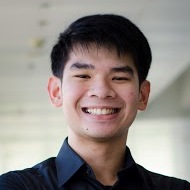
\includegraphics[width=0.2\columnwidth]{Jarabelo}
\documentAuthor{firstname3} \ \documentAuthor{surname3} \ is currently studying B. S. Computer Engineering in De La Salle University, Malate, Manila, Philippines. 

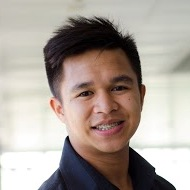
\includegraphics[width=0.2\columnwidth]{Uy}
\documentAuthor{firstname4} \ \documentAuthor{surname4} \ is a forth year engineering student and currently taking up Bachelor of Science in Computer Engineering at De La Salle University - Manila, Philippines. He is knowledgeable in database systems, programming languages such as C, CSS, Java, HTML, MySQL, PHP and Verilog, and has developed several electronic circuits that utilizes the PIC microcontroller. His research interest includes automation, environment friendly technologies and radio frequency identification technologies.

%\vfill
%}


\fi
\cleardoublepage

%%%%%%%%%%%%%%%%%%%%%%%%%%%%%%%%%%%%%%%%%%%%%%%%
\ifIndex
	\printindex
\fi
\cleardoublepage

\end{document}
